%% AAAI-27 submission -- anonymous (double-blind) version.
%% Build: pdflatex main ; bibtex main ; pdflatex main ; pdflatex main
%% Camera-ready: see README.md (switch [submission] -> {aaai2027}; restore authors/links/IRB).
\documentclass[letterpaper]{article} % DO NOT CHANGE THIS
\usepackage[submission]{aaai2027}  % DO NOT CHANGE THIS
\usepackage[hyphens]{url}  % DO NOT CHANGE THIS
\usepackage{graphicx} % DO NOT CHANGE THIS
\urlstyle{rm} % DO NOT CHANGE THIS
\def\UrlFont{\rm}  % DO NOT CHANGE THIS
\usepackage{natbib}  % DO NOT CHANGE THIS AND DO NOT ADD ANY OPTIONS TO IT
\usepackage{caption} % DO NOT CHANGE THIS AND DO NOT ADD ANY OPTIONS TO IT
\frenchspacing  % DO NOT CHANGE THIS
% Math + tables (standard, allowed).
\usepackage{amsmath}
\usepackage{amssymb}
\usepackage{booktabs}
\usepackage{array}
\pdfinfo{
/TemplateVersion (2027.1)
}
\setcounter{secnumdepth}{2} % number sections and subsections (so \ref{sec:...} resolves)

\title{Cross-Age Face Verification from Mined Same-Person Social-Media Pairs}

\author{
    Anonymous Submission
}
\affiliations{
    %% Camera-ready: replace with real author(s) and affiliation(s); see README.md.
}

\begin{document}
\maketitle

\begin{abstract}
Cross-age face verification---deciding whether two photographs taken years apart depict the same person---is hard, and longitudinal training data are scarce. We ask a \emph{data-centric} question: can supervision for age invariance be obtained without a manually labeled longitudinal dataset? We show that multi-photo ``then/now'' social-media posts supply weak \emph{same-person} longitudinal pairs with no manual identity or age labels (a large language model parses captions and embedding clustering forms persons; we audit these components, including a small manual validation), and that fine-tuning a deliberately weak recognizer on them induces \emph{transferable, targeted} large-gap robustness. On the external benchmark FG-NET, large-gap ($\geq$25-year) ROC-AUC rises \textbf{from 0.736 to 0.848} ($+$0.112 $\pm$ 0.001 over three seeds; DeLong $p<10^{-19}$), at the cost of $-$0.019 LFW accuracy and \emph{substantial} low-FAR degradation---a targeted retrieval gain, not a general-verifier upgrade. Our central, bounded claim is that, within this weak-backbone attribution protocol, the \emph{data source}---not the choice among the objectives we test---accounts for most of the gain: a pair-contrastive objective matches an ArcFace-margin one (0.848 vs.\ 0.851). The gain is driven by the same-person pairing (caption age anchors add only $+$0.009), is mechanistically tied to removing an age shortcut, beats a real re-aging model under a gap-parity control, and transfers to an independent non-VK platform.
\end{abstract}

\section{Introduction}\label{sec:intro}
Cross-age face verification arises in archival retrieval, account recovery, and authorized search for missing persons. The challenge lies not in discriminating among arbitrary individuals but in distinguishing \emph{the same person across age} from \emph{different people of similar age and appearance}. Annotating longitudinal identity pairs (one individual across many years) is costly, and such data remain scarce, which constrains supervised approaches; recent work continues to report weak cross-dataset generalization and a shortage of high-quality longitudinal data.

\textbf{Hypothesis.} A multi-photo ``then/now'' post showing one person at different ages yields $\binom{n}{2}$ positive identity pairs without manual annotation; a caption stating ages adds a secondary age anchor. The same-person pairing is the operative signal (an ablation isolates the age anchor at a marginal $+$0.009); this is a scalable, weakly/naturally-supervised signal of cross-age identity, and fine-tuning a weak recognizer on it should transfer to external benchmarks.

\textbf{Contributions (bounded).}
(1)~A weakly/naturally-supervised (no manual id/age labels) longitudinal signal mined from social posts---same-person identity pairs, with caption age anchors only a secondary cue.
(2)~A rigorous \emph{attribution protocol} (one weak trainable backbone, frozen vs.\ fine-tuned, external evaluation) that isolates the contribution of \emph{data} from network capacity.
(3)~Mutually reinforcing controls (loss family, architecture, source community, training objective, real-vs-synthetic, shortcut diagnosis, cross-platform transfer) supporting the bounded claim that, within this protocol and across the objectives tested, the data contributes more to the large-gap gain than the choice among loss families.
(4)~A curation pipeline with an audit of its automatic components, and the finding that naive positive counts are inflated about $2\times$ by near-duplicate frames.
The novelty is data-centric rather than architectural---a new \emph{origin of supervision}---and should be evaluated accordingly. A supplementary technical appendix reports the controls and audits deferred for space.

\section{Related Work and Positioning}\label{sec:related}
Three lines of prior work are most relevant. \emph{Discriminative age-invariant FR on labeled data:} OE-CNN (orthogonal embedding decomposition)~\cite{wang2018oecnn}, DAL (decorrelated adversarial learning)~\cite{wang2019dal}, and MTLFace (multi-task recognition, age synthesis and attention decomposition)~\cite{huang2021mtlface} achieve strong accuracy but are trained on datasets with \emph{manual identity and age labels} (CACD~\cite{chen2014cacd}, MORPH~\cite{ricanek2006morph}, AgeDB~\cite{moschoglou2017agedb}, FG-NET~\cite{panis2016fgnet}). \emph{Cross-age contrastive with synthetic samples:} CACon~\cite{wang2024cacon} adds a synthesized cross-age sample and a triplet loss; OrdCon~\cite{wang2025ordcon} uses order-enhanced contrastive learning. \emph{Synthetic aging for robustness:} systematic studies show synthetic aging helps only partially~\cite{yao2024synthageing}. Generic self-supervised FR (SimCLR-style augmentation~\cite{chen2020simclr}) lacks identity anchors across time. We instead mine the structure ``one post $=$ one person at different ages'' as a label-free positive-pair generator (a per-method positioning table is in the supplement). We report on the canonical cross-age benchmarks of these methods (AgeDB-30, CALFW~\cite{zheng2017calfw}, FG-NET; CALFW is a harder, age-gapped LFW~\cite{huang2007lfw}). The goal is \emph{not} to surpass the absolute state of the art (we use a weak backbone for clean attribution) but to quantify the magnitude and transferability of the gain from a naturally-supervised source; Sec.~\ref{sec:res-main} trains the canonical SOTA objective on our data directly.

\section{Data: Naturally-Anchored Longitudinal Pairs}\label{sec:data}
\textbf{Source.} Two public ``then/now'' multi-photo communities on VK (one platform, Russian-language context). Faces are detected and aligned with a 5-point ArcFace template (InsightFace RetinaFace~\cite{deng2020retinaface}, \texttt{buffalo\_l}). A \emph{usable} face passes detection-score, minimum-size, blur, and single-target checks (Sec.~\ref{sec:method}). The raw mined corpus is summarized in Table~\ref{tab:scale}.

\begin{table*}[t]
\centering
\small
\begin{tabular}{@{}lrrrrr@{}}
\toprule
Stage & Posts & Photos & Usable faces & Persons (groups) & Positive pairs \\
\midrule
Raw mined (2 communities) & 44{,}609 & 84{,}147 & 49{,}606 & 21{,}848 & 65{,}897 \\
\textbf{After curation} & --- & --- & \textbf{40{,}586} & \textbf{21{,}427} & \textbf{31{,}865} \\
\bottomrule
\end{tabular}
\caption{Dataset scale (raw mined) and after curation. Removing near-duplicate frames roughly halves the positive count.}
\label{tab:scale}
\end{table*}

\textbf{Age extraction.} Captions are parsed by regular expressions (Russian patterns plus the slash format ``6/18/21'') and by a large language model (LLM). Across all 33{,}697 multi-photo captions the LLM broadens and regularizes extraction relative to regex---it avoids reading calendar years or gaps as ages and recovers second ages---disagreeing on 27.2\% of posts, overwhelmingly LLM-favoring; on a 100-caption manual gold subset the LLM matched the human reading on 89\% vs.\ regex 71\% (supplement). We do not treat LLM output as ground truth: downstream, explicit age anchors contribute only marginally (Sec.~\ref{sec:res-main}).

\textbf{Persons and leakage-safe split.} A naive ``one post $=$ one identity'' undercounts: a person recurs across posts. We cluster post-groups into persons by embedding similarity (cosine $\geq$ 0.85), giving 21{,}848 persons from 27{,}487 post-groups ($\approx$20\% recurrence), and split \emph{by person} (not by post). Manual inspection showed cosine does not separate look-alikes from same-person in the 0.55--0.8 band, so the merge threshold is deliberately conservative.

\textbf{Auditing the supervision.} The automatic components are potential hidden label noise, audited three ways: LLM-vs-regex age agreement; within-person apparent-gender consistency as an inexpensive multi-person detector; and a \emph{small} manual validation (one annotator) that \emph{sanity-checks} the pipeline (age, group integrity, pair and merge precision $0.93$--$0.96$; supplement). With a single annotator and no inter-annotator $\kappa$ this \emph{supports} but does not \emph{certify} the supervision; a large multi-annotator audit is beyond our resources, so residual noise is acknowledged as a limitation (Sec.~\ref{sec:limitations}).

\textbf{Curation and its largest finding.} We apply per-person apparent gender/age aggregation, LLM group-integrity validation (92.8\% single-person), and near-duplicate dedup within each person (cosine $\geq$ 0.97). Because the number of positives is quadratic in faces per group, removing near-duplicates cut the positive count from 65{,}897 to 31{,}865 ($-$52\%): \textbf{about half of the raw ``positives'' were duplicate frames} (a single shoot, burst, or repost) inflating internal metrics. After curation the frozen internal baseline drops (our.25+ $0.705\!\rightarrow\!0.640$), exposing a harder, more representative benchmark; external benchmarks are unaffected. The reduction is stable across dedup thresholds $0.93$--$0.97$ (supplement). Provenance, rights and governance fields are stored per item; a full datasheet~\cite{gebru2021datasheets} accompanies the controlled-access release (see the Ethical Statement).

\section{Method, Protocol and Statistics}\label{sec:method}
\textbf{Attribution protocol.} Comparing an adapter on top of a \emph{frozen} strong ArcFace against frozen ArcFace is invalid (the adapter merely deforms near-perfect embeddings). Instead we use \emph{one weak trainable backbone} (FaceNet InceptionResnetV1~\cite{schroff2015facenet}, CASIA-WebFace) and compare (a)~frozen $\rightarrow$ benchmark metric vs.\ (b)~soft fine-tuning of the head on our pairs $\rightarrow$ benchmark metric, with a margin contrastive loss on aligned crops. \emph{Evaluation is on external benchmarks} (LFW, AgeDB-30, CALFW, FG-NET) for a clean attribution of transfer; the internal test (\texttt{our.*}) is a secondary in-domain diagnostic. Backbone strength is varied (Sec.~\ref{sec:res-headroom}) to map where the data helps. The design trades absolute performance for \emph{causal attribution}.

\textbf{Backbones and metrics.} FaceNet (weak); ArcFace iResNet-50~\cite{deng2019arcface} (weak, different architecture); AdaFace IR-50/IR-101~\cite{kim2022adaface} and ArcFace iResNet-100 (strong; a clean depth control). We report LFW (10-fold accuracy), AgeDB-30 and CALFW (ROC-AUC and accuracy), and FG-NET (ROC-AUC overall and on the large-gap $\geq$25-year subset), distinguishing \emph{threshold-free} metrics (ROC-AUC) from \emph{threshold-based} ones (accuracy, TAR@FAR).

\textbf{Statistics.} The \emph{primary endpoint} is FG-NET large-gap ROC-AUC, with the null hypothesis that fine-tuning does not improve it over frozen (gain $\leq 0$); AgeDB-30, CALFW and the internal cross-age test are secondary, and easy LFW accuracy is a forgetting control. The headline gain is mean $\pm$ std over three seeds. We report bootstrap CIs, EER and TAR@FAR (the internal test additionally uses an identity-level, person-resampling bootstrap), DeLong's test for two \emph{correlated} ROC curves~\cite{delong1988}, a paired permutation test, and a Holm correction across the stratified fairness tests (full operating-point tables in the supplement). All headline experiments use the curated data (21{,}427 groups, 40{,}586 faces, 31{,}865 positives; by-person split with balanced negatives).

\section{Results}\label{sec:results}
\subsection{Main Effect and Supervision-Source Ablation}\label{sec:res-main}
The weak FaceNet, softly fine-tuned on our pairs, raises FG-NET large-gap ROC-AUC \textbf{0.736 $\rightarrow$ 0.848} ($+$0.112 $\pm$ 0.001), while easy LFW falls only $-$0.019 and AgeDB-30/CALFW move negligibly (Table~\ref{tab:main}). An ablation isolates the source: same-post pairs use no manual labels and deliver almost all of the gain; adding explicit age anchors contributes only \textbf{$+$0.009} on the 25+ bucket. The method is therefore \emph{weakly supervised by naturally occurring same-post co-occurrence}, with age supervision marginal.

\begin{table*}[t]
\centering
\small
\begin{tabular}{@{}lcccc@{}}
\toprule
Metric & Frozen & $+$pairs (mean $\pm$ std) & Gain & (Pre-clean gain) \\
\midrule
FG-NET large-gap & 0.7361 & 0.8484 $\pm$ 0.0007 & \textbf{$+$0.1124} & $+$0.1215 \\
FG-NET ROC & 0.8955 & 0.9230 $\pm$ 0.0006 & $+$0.0275 & $+$0.0277 \\
our.25+ (internal) & 0.6403 & 0.8348 $\pm$ 0.0027 & \textbf{$+$0.1946} & $+$0.1677 \\
our.overall (internal) & 0.8363 & 0.9163 $\pm$ 0.0009 & $+$0.0801 & $+$0.0764 \\
LFW accuracy & 0.9688 & 0.9503 $\pm$ 0.0031 & $-$0.0185 & $-$0.0283 \\
AgeDB-30 ROC & 0.9530 & 0.9462 $\pm$ 0.0013 & $-$0.0068 & $-$0.0155 \\
CALFW ROC & 0.9482 & 0.9489 $\pm$ 0.0014 & $+$0.0007 & $-$0.0030 \\
\bottomrule
\end{tabular}
\caption{Main result: weak FaceNet frozen vs.\ $+$pairs, three seeds, curated data (pre-clean gain shown for reference). The gain is concentrated on the FG-NET large-gap subset.}
\label{tab:main}
\end{table*}

Bootstrap confidence intervals (seed 42) confirm the primary endpoint: FG-NET large-gap rises from 0.736~[0.70, 0.78] to 0.848~[0.82, 0.88] with \emph{non-overlapping} 95\% CIs; the equal-error rate nearly halves (0.335$\to$0.219) and TAR@FAR$=$1\% nearly doubles (0.21$\to$0.39). Because bootstrap-CI overlap ignores the samples the two models share, we confirm the endpoint with DeLong's test for correlated ROC curves~\cite{delong1988}: on FG-NET large-gap $z=9.3$, $p=1.4\times10^{-20}$ ($\Delta$AUC 95\% CI $[+0.088,+0.135]$); a $10^4$-fold paired permutation test agrees ($p<10^{-4}$). The same test shows the gain is \emph{targeted}: AgeDB-30 decreases slightly ($-$0.008, $p=4\times10^{-6}$) and CALFW is unchanged ($p=0.95$). Operating points (Table~\ref{tab:stats}) make the trade-off concrete: large-gap AUC and TAR@1\% rise sharply, while easy-benchmark low-FAR points (LFW TAR@0.1\%) degrade.

\begin{table*}[t]
\centering
\small
\begin{tabular}{@{}lccccc@{}}
\toprule
Benchmark & Frozen AUC [95\% CI] & $+$pairs AUC [95\% CI] & EER (fr.$\to$$+$p.) & TAR@1\% & TAR@0.1\% \\
\midrule
FG-NET large-gap & 0.736 [0.70, 0.78] & \textbf{0.848 [0.82, 0.88]} & 0.335$\to$0.219 & 0.209$\to$0.386 & 0.074$\to$0.154 \\
FG-NET overall & 0.896 [0.89, 0.90] & 0.922 [0.92, 0.93] & 0.186$\to$0.151 & 0.502$\to$0.562 & 0.315$\to$0.308 \\
AgeDB-30 & 0.953 [0.95, 0.96] & 0.945 [0.94, 0.95] & 0.115$\to$0.126 & 0.525$\to$0.510 & 0.285$\to$0.309 \\
CALFW & 0.948 [0.94, 0.95] & 0.948 [0.94, 0.95] & 0.116$\to$0.117 & 0.580$\to$0.624 & 0.213$\to$0.320 \\
LFW (AUC) & 0.994 [0.99, 1.00] & 0.987 [0.98, 0.99] & 0.032$\to$0.052 & 0.940$\to$0.869 & 0.858$\to$0.575 \\
\bottomrule
\end{tabular}
\caption{Operating points and 95\% bootstrap CIs (FaceNet frozen vs.\ $+$pairs, seed 42); the internal test additionally uses an identity-level bootstrap (text). LFW is shown as ROC-AUC for consistency.}
\label{tab:stats}
\end{table*}

\textbf{Objective invariance.} Training the canonical modern-FR margin objectives---ArcFace, CosFace and SphereFace identity classification~\cite{deng2019arcface} (the core of OE-CNN/MTLFace)---on our naturally-supervised identities, same backbone and protocol, the contrastive, ArcFace and CosFace objectives \textbf{coincide} on the primary endpoint (0.848 / 0.851 / 0.843, within $\pm$0.006); only SphereFace, hardest to optimize on 2--3-shot identities without $\lambda$-annealing, trails (0.801). A noise-robust sub-center ArcFace~\cite{deng2020subcenter} also lands at 0.851---explicit label-noise machinery adds nothing on the \emph{curated} pairs. We draw the bounded conclusion that, within this protocol and among the objectives tested, the \emph{data source} accounts for more of the gain than the objective choice (Table~\ref{tab:objective}).

\begin{table}[t]
\centering
\setlength{\tabcolsep}{3pt}
\small
\begin{tabular}{@{}lcccc@{}}
\toprule
Objective & FG-NET l.g. & our.25+ & LFW & AgeDB-30 \\
\midrule
Frozen & 0.736 & 0.640 & 0.969 & 0.953 \\
$+$pairs (contrastive) & 0.848 & 0.838 & 0.946 & 0.945 \\
$+$ArcFace & \textbf{0.851} & 0.868 & 0.952 & 0.947 \\
$+$ArcFace, sub-center & 0.851 & 0.869 & 0.951 & 0.947 \\
$+$CosFace & 0.843 & 0.860 & 0.952 & 0.945 \\
$+$SphereFace & 0.801 & 0.699 & 0.950 & 0.943 \\
\bottomrule
\end{tabular}
\caption{Objective comparison (FaceNet, curated): contrastive, ArcFace and CosFace coincide on the FG-NET large-gap primary endpoint; a noise-robust sub-center ArcFace adds nothing; SphereFace (no $\lambda$-annealing) trails on sparse few-shot identities.}
\label{tab:objective}
\end{table}

\subsection{Real Pairs Outperform Synthetic Aging}\label{sec:res-synth}
Replacing real positives with synthetically aged versions---a domain proxy and a real re-aging network (FRAN~\cite{zoss2022fran})---underperforms real pairs, and at FRAN's default \emph{wide-gap} setting even \emph{degrades} below frozen (FG-NET large-gap 0.727; Table~\ref{tab:synth}). Identity-preserving aging reproduces texture artifacts rather than genuine longitudinal variation (pose, camera, era). A native-resolution control rules out a crop artifact: re-cropping a train subset at 512~px directly from the raw images and re-aging leaves the result unchanged (0.771 vs.\ 0.778). A gap-parity control sharpens this: FRAN ages to a wide 33--70-year gap whereas real pairs have a median gap of 9~years; matching the synthetic gap to the real distribution lifts FRAN to \textbf{0.759}---a modest positive in line with reported synthetic-aging gains~\cite{yao2024synthageing}---yet real pairs (0.848) still lead by $+$0.089. Real mined pairs beat even a \emph{gap-matched} re-aging model.

\begin{table}[t]
\centering
\small
\begin{tabular}{@{}lcccc@{}}
\toprule
Metric & Frozen & $+$real & syn-FRAN & FRAN-gm \\
\midrule
FG-NET large-gap & 0.736 & \textbf{0.848} & 0.727 & 0.759 \\
our.25+ & 0.640 & \textbf{0.838} & 0.549 & 0.622 \\
\bottomrule
\end{tabular}
\caption{Real vs.\ synthetic positives (FaceNet, curated). FRAN-gm matches the synthetic age-gap to the real-pair distribution (median 9~y).}
\label{tab:synth}
\end{table}

\subsection{Headroom and Data Scaling}\label{sec:res-headroom}
The gain reproduces on FaceNet, ArcFace iResNet, and AdaFace IR-50/IR-101 (three loss families, two architectures) and \emph{monotonically decreases with frozen strength} (Fig.~\ref{fig:headroom}); a clean depth control (AdaFace IR-50 $\rightarrow$ IR-101) confirms it. Strong saturated backbones do not improve and forget slightly under fine-tuning; a gentler learning rate halves the forgetting but does not convert it into a gain. The contribution is therefore specific to weak and medium backbones with cross-age headroom---a limitation we state explicitly (Sec.~\ref{sec:limitations}). Varying the fraction of training identities (val/test fixed), the gain saturates early: \textbf{$\approx$96\% of the full FG-NET large-gap gain is reached with only 10\% of identities} ($\approx$1{,}500), plateauing from 25\% (Fig.~\ref{fig:scaling}; each point mean $\pm$ std over three seeds). The signal is data-efficient; further gains require \emph{harder} data (larger gaps, hard positives) rather than merely more volume.

\begin{figure}[t]
\centering
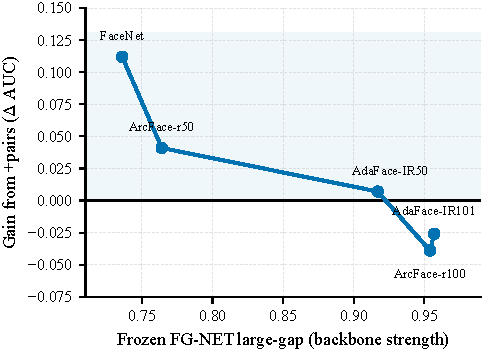
\includegraphics[width=\columnwidth]{figures/fig_headroom.pdf}
\caption{Headroom curve: the $+$pairs gain on FG-NET large-gap shrinks monotonically as the frozen backbone strengthens, crossing zero for strong saturated models.}
\label{fig:headroom}
\end{figure}

\begin{figure}[t]
\centering
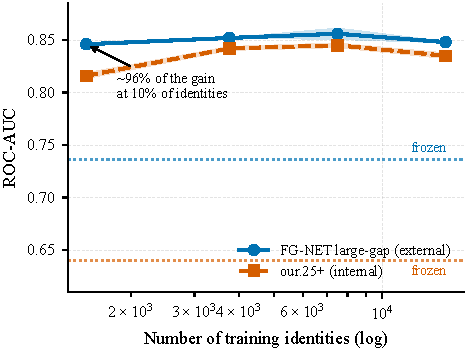
\includegraphics[width=\columnwidth]{figures/fig_scaling.pdf}
\caption{Data-scaling law: external (FG-NET large-gap) and internal (our.25+) ROC-AUC vs.\ training identities (log scale). About 96\% of the gain is reached at 10\% of identities; shaded bands are $\pm$1 std over three seeds, dashed lines the frozen baselines.}
\label{fig:scaling}
\end{figure}

\subsection{Mechanism: the Age Shortcut}\label{sec:res-shortcut}
Under age-matched negatives (same age bucket, different people), frozen accuracy on the internal 25+ test falls from 0.640 to 0.517 (\textbf{near the chance level of 0.5}), and real pairs restore it to \textbf{0.838} (Fig.~\ref{fig:shortcut})---direct evidence that frozen models discriminate cross-age pairs largely by \emph{age}, whereas our pairs induce discrimination by \emph{identity}. A linear probe refines this representationally: apparent age stays well decodable from the identity embedding for \emph{all} models ($\approx$0.63--0.65 balanced accuracy $\gg$ 0.25 chance) and changes only slightly, while identity AUC rises sharply (0.836 $\rightarrow$ 0.916)---the method learns an invariant \emph{metric} (the cosine stops relying on the age axis), not an age-free representation; explicit adversarial disentanglement reduces leakage no further (supplement).

\begin{figure}[t]
\centering
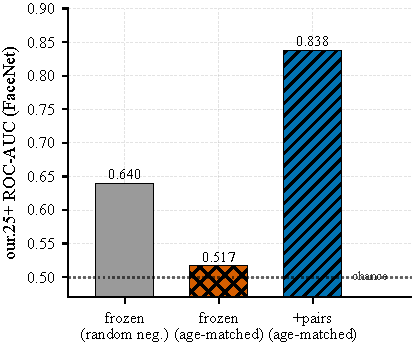
\includegraphics[width=0.86\columnwidth]{figures/fig_shortcut.pdf}
\caption{The age shortcut: on an identity-only test (age-matched negatives) the frozen model falls to near-chance; fine-tuning on our pairs restores discrimination by identity.}
\label{fig:shortcut}
\end{figure}

\subsection{Cross-Platform and Cross-Source Transfer}\label{sec:res-cross}
Training on one VK community and testing on the held-out other transfers the gain (external FG-NET large-gap $+$0.113, essentially identical to the within-source $+$0.112). A stronger external check is whether the \emph{source} generalizes beyond its platform. Applying the \emph{identical} mining protocol to an independent, non-VK community---the Reddit board r/PastAndPresentPics (same ``then/now'' format, same LLM parser)---and evaluating the VK-trained $+$pairs model with \emph{no} Reddit data in training on 1{,}575 Reddit pairs raises overall ROC-AUC \textbf{0.718 $\rightarrow$ 0.749} ($+$0.031, near-disjoint 95\% CIs). The transfer is \emph{bidirectional}: a backbone trained on \emph{only} a small 220-person Reddit source (a pilot, not a headline) also helps on VK (FG-NET large-gap $+$0.047). The gain is smaller than within-VK (a noisier, partly collage-derived set), so we read it as confirming the source generalizes beyond its platform, not as a SOTA claim. Figure~\ref{fig:external} shows the $+$pairs gain stays \emph{positive across all three} external evaluations, shrinking on harder/noisier sets.

\begin{figure}[t]
\centering
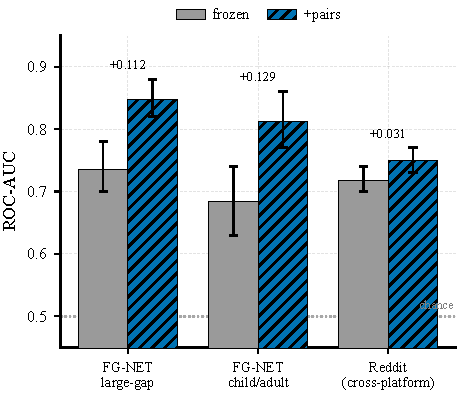
\includegraphics[width=\columnwidth]{figures/fig_external.pdf}
\caption{External generalization. The $+$pairs gain over frozen (95\% CIs) holds across three independent evaluations---FG-NET large-gap, a child$\leftrightarrow$adult FG-NET subset, and the cross-platform Reddit set---each well above chance, largest on the in-protocol FG-NET sets and smaller (but positive) on the noisier Reddit set.}
\label{fig:external}
\end{figure}

\textbf{Apparent-demographic audit.} Stratifying by \emph{apparent} gender/age of the pair anchor (estimated, not self-identified), no group degrades and every gain is significant (95\% paired-bootstrap CI $>$ 0; supplement). The largest gain is for the youngest group 0--17 (0.750 $\rightarrow$ 0.880, $+$0.130)---the method strengthens where the base model is weakest---corroborated on an \emph{independent} child$\leftrightarrow$adult FG-NET subset ($+$0.129, non-overlapping CIs). At a matched $\approx$1\% FMR, $+$pairs lowers the false-non-match rate in every apparent stratum. We avoid the word ``fair'' as a solved property: the source is apparent-female-skewed (76.7\%) and attributes are apparent, not legal categories.

\section{Discussion}\label{sec:discussion}
The contribution is a scalable, weakly/naturally-supervised source of longitudinal supervision that teaches transferable cross-age robustness which synthetic aging cannot replace and explicit age supervision does not explain. Reinforcing controls---loss family, architecture, source community, objective, and a noise-robust margin---converge on a bounded conclusion: within this protocol, the \emph{data source} accounts for more of the large-gap gain than the choice of objective. Crucially, the improvement is a \emph{targeted} large-gap gain, not a drop-in upgrade to a general verifier: low-FAR operating points on easy benchmarks degrade (LFW TAR@FAR$=$0.1\% falls $0.858 \rightarrow 0.575$), so deployment should be scoped to the large-gap cross-age regime.

\textbf{Scope of the claims.} \emph{Established (within this attribution protocol):} (i)~the mined pairs improve large-gap cross-age verification on FG-NET (primary endpoint, non-overlapping 95\% CIs) and the internal 25+ test; (ii)~the gain transfers across the two source communities, to an independent child$\leftrightarrow$adult FG-NET subset, and to a non-VK platform; (iii)~real pairs \textbf{outperform synthetic aging}, including under native-resolution and gap-parity controls; (iv)~the gain is invariant across the contrastive, ArcFace and CosFace objectives; (v)~it is mechanistically tied to \textbf{removing an age shortcut}; (vi)~roughly half of the raw positive pairs were near-duplicate frames. \emph{Not established / out of scope:} the effect is not a uniform verification gain (low-FAR operating points degrade); strong saturated backbones do not improve; a larger non-VK \emph{training} source with multi-seed CIs remains future work; we do not reproduce a full SOTA pipeline, only its shared margin objective; the fairness audit uses apparent attributes only and lacks a multi-annotator $\kappa$.

\section{Limitations}\label{sec:limitations}
\begin{itemize}
\item \textbf{Backbone dependence:} the gain concentrates in weak/medium backbones; strong saturated models do not improve and slightly forget.
\item \textbf{External validity:} two VK communities, one platform, one language/cultural context; apparent-female-skewed (76.7\%); sparse at apparent age 45+. Transfer is shown between two VK sources, to standard external benchmarks, and to a small independent Reddit then/now test; this does not establish platform-agnostic generalization.
\item \textbf{Apparent attributes only} in the fairness audit (estimated, not self-identified gender/ethnicity), and no human-audited inter-annotator $\kappa$ (a large manual audit is labor-intensive and beyond our resources).
\item \textbf{Weakly supervised, not label-free:} an LLM parses ages and validates group integrity and clustering forms persons---audited but a residual hidden-noise source.
\item \textbf{Benchmark scale and age:} the field-standard cross-age suite (AgeDB-30, CALFW, FG-NET) fixes comparability but inherits limited scale/age; a larger non-VK longitudinal set remains useful future work.
\end{itemize}

\section*{Ethical Statement}
This is a sensitive biometric study; we treat governance as a first-class component. Permitted use is restricted to controlled / consent-based / human-reviewed applications (rights-cleared archives and family photos, authorized humanitarian search, account recovery); the system outputs candidates for human review, never an automatic decision. This is a \emph{research-only} study---nothing is deployed and \emph{no public biometric database is released}. Forbidden: mass identification, de-anonymization, surveillance, and any processing of minors' data without a legal basis.

\emph{Ethical approval.} This study was reviewed and approved by the authors' institutional research ethics committee; the committee name, protocol number and approval date are withheld here to preserve anonymity and will be provided in the camera-ready version. \emph{Consent.} Because the data are drawn from public posts with no feasible channel to contact subjects, individual informed consent for participation and publication was not obtained; we rely on a scientific-research legal basis with the de-identification safeguards below, and note that official API access and voluntary public posting do not by themselves authorize biometric processing (cf.\ GDPR Art.~9 special-category data~\cite{gdpr2016} and national biometric-consent law). We report this gap transparently rather than claiming full compliance.

\emph{De-identification and release.} We \emph{do not release raw face images or raw posts}. The public release is restricted to code, configurations, the pseudonymized benchmark protocol and aggregate statistics. Because a face embedding is itself a comparable \emph{biometric template} and salted identifier hashes do not render it anonymous, trained weights and derived embeddings are made available \emph{only} under controlled access (Data Use Agreement; research-only; no re-identification). Platform identifiers are replaced by salted hashes; captions/comments are excluded; only an age bucket and a pseudonymous person ID are kept. Minor-age items are withheld from any release absent an explicit legal framework and verifiable guardian consent. A Data Protection Impact Assessment, a full datasheet~\cite{gebru2021datasheets} and a takedown / deletion-on-request procedure accompany the release.

\textbf{Reproducibility.} We release all scripts, configurations and versioned LLM prompts; raw face images and posts are withheld, so data-mining replication is partial (we release cached LLM outputs for deterministic replay). The entire study runs on a single laptop (one 6~GB GPU). A reproducibility checklist accompanies the submission.

\bibliography{refs}

\end{document}
